\section{December forecast}

The chart rows have no market index and no coordinates. We look the coordinates up from the city list, and take
each day's market index as the mean over that day's loads in \texttt{validation.csv}.

The forecast runs from \usd{\DecMin} to \usd{\DecMax} and ends at \usd{\DecLast} on December 31
(Figure~\ref{fig:december}). The weekly wave follows the market index. The slow rise is the drift plus the
quarter-end ramp.

\begin{figure}[H]
  \centering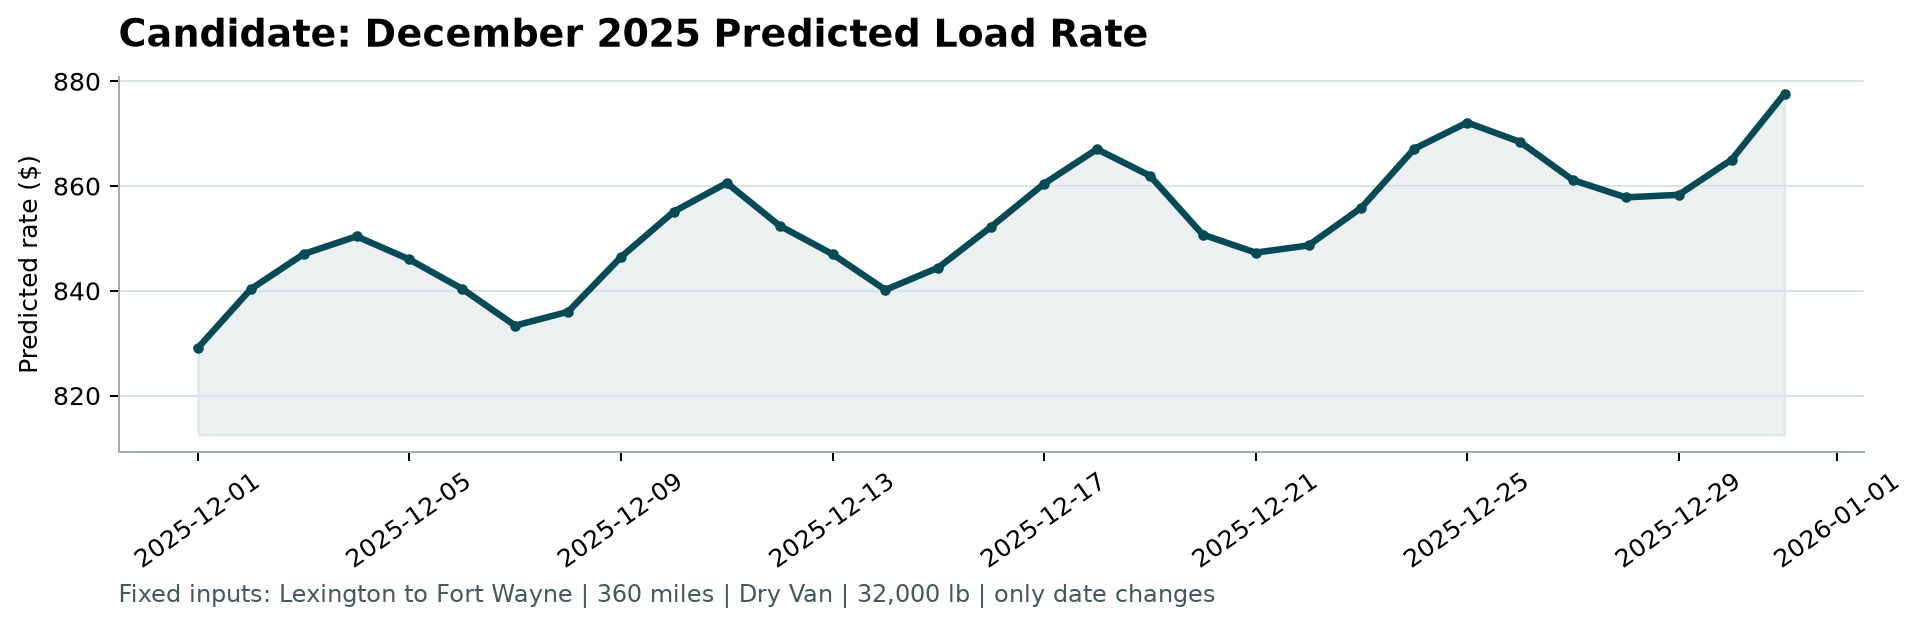
\includegraphics[width=0.95\linewidth]{candidate_december.png}
  \caption{The December chart produced by the assessment's own \texttt{score.py}.}\label{fig:december}
\end{figure}

\textbf{How much rests on the quarter-end ramp?} December has never been observed. The ramp was seen in March, June
and September, and the model assumes it recurs. Without it, December 31 would be \usd{\DecLastNoRamp} instead of
\usd{\DecLast}. If the December market index were unknown and held at its October mean, the line would be a smooth
\usd{\DecFlatMin} to \usd{\DecFlatMax} (Figure~\ref{fig:sensitivity}).

\begin{figure}[H]
  \centering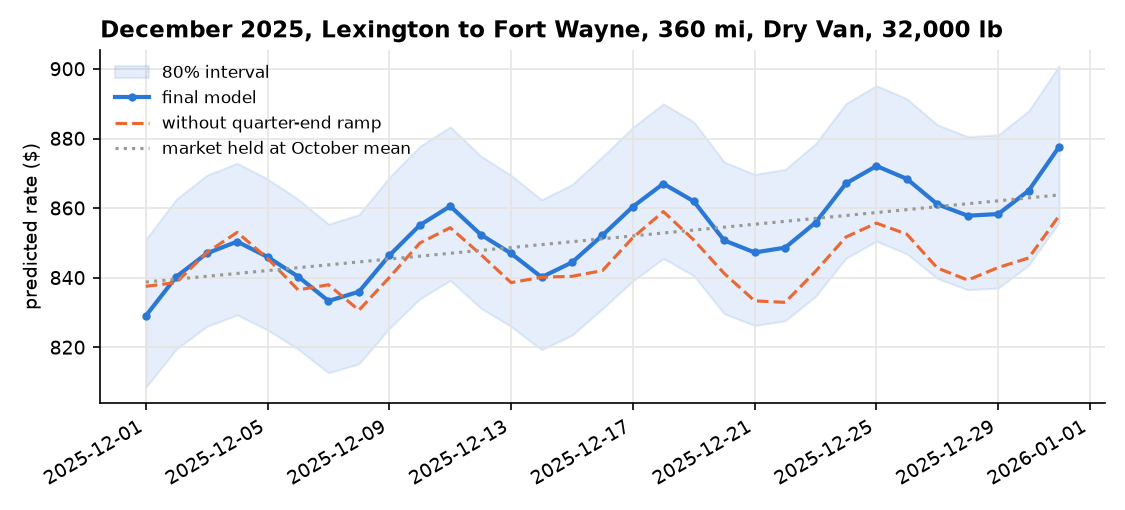
\includegraphics[width=0.9\linewidth]{december_sensitivity.png}
  \caption{December forecast with its 80\% interval, without the quarter-end ramp, and with the market held at its
  October mean.}\label{fig:sensitivity}
\end{figure}
